\chapter{Test}
\label{cha:Test}
In diesem Kapitel werden die Anforderungen an die Webanwendung anhand eines Integrationstests überprüft. Zu diesem Zweck wird ein Testszenario beschrieben und der Versuchsaufbau erläutert. Das zu erwartende Ergebnis wird anschließend mit dem tatsächlich eingetretenen Resultat abgeglichen.

\section{Vorgehensweise}
\subsection{Verfahren}

Aus zeitlichen Gründen konnten keine softwaregestützten Tests implementiert werden. Stattdessen wurden die in Abschnitt \ref{sec:Funktionale Anforderungen} gestellten funktionalen Anforderungen mit Hilfe eines manuell durchgeführten Integrationstests überprüft. Ein Integrationstest kennzeichnet sich durch eine aufeinander abgestimmte Reihe von Einzeltests, die dazu dienen, verschiedene voneinander abhängige Komponenten eines Systems im Zusammenspiel miteinander zu testen. Die erstmals im gemeinsamen Kontext zu testenden Komponenten haben im Idealfall bereits Modultests erfolgreich bestanden und sind für sich fehlerfrei funktionsfähig. Da die fehlerfreie Funktionsfähigkeit der einzelnen Module der realisierten Webanwendung nicht gewährleistet werden kann, ist die Durchführung eines Integrationstests ein riskantes Unterfangen und lässt Zweifel an der Aussagefähigkeit eines möglichen Ergebnisses zu.

Um aber zumindest das Erreichen des Gesamtziels der prototypischen Implementierung zu belegen, wird in Abschnitt \ref{sec:test:Planung und Ablauf} ein Testszenario beschrieben, das die in Abschnitt \ref{sec:Funktionale Anforderungen} definierten funktionalen Anforderungen abdeckt.

\subsection{Testszenario und Durchführung}
\label{sec:test:Planung und Ablauf}

\subsubsection{Testszenario} 

Für das gesetzte Ziel, alle funktionalen Anforderungen in dem durchzuführenden Integrationstest abzudecken, wurde nachfolgend ein komplexes Testszenario erarbeitet.
Über die Webanwendung soll ein neuer Filter vom Typ Boolean angelegt werden. An diesen Filter sollen mehrere Properties gespeichert werden, die ebenfalls neu angelegt werden. Diesen Properties werden jeweils wiederum mehrere Models zugewiesen. Zusätzlich soll das dabei entstehende Filtersteuerelement über die implementierte Drag-and-Drop Funktionalität verschoben werden. Anschließend werden die Daten exportiert, um sie im FlowConfigurator anzuzeigen. Der Export und Import der Daten in die FlowConfigurator Software wird dabei über ein Kommando realisiert, das von der netbase GmbH entwickelt und bereitgestellt wurde. Der Export der Daten und die Wiedernutzbarmachung im FlowConfigurator ist nicht Teil der Anforderungen an die realisierte Webanwendung.

\subsubsection{Durchführung}

Vor der Durchführung des Testszenarios wurde die Datenbank auf ihren Ursprungszustand zurückgesetzt. Anschließend wurde stichprobenartig überprüft ob durch das Zurücksetzen der Datenbank etwaige Fehler in der Webanwendung entstanden sind. Nachdem eine saubere Ausgangsbasis für den anstehenden Integrationstests verifiziert werden konnte, wurde mit der Durchführung begonnen.

Es wurde ein neuer Filter mit der Bezeichnung \emph{Test}, innerhalb der Produktfamilie \emph{Variable area flowmeter (Rotameter)} und der Produktlinie \emph{RAMC}, angelegt. Der Filter ist außerdem vom Typ \emph{Boolean} und gehört der Gruppe der \emph{Basisfilter} an. Anschließend wurden Properties mit der Bezeichnung \emph{Test Property 1} und \emph{Test Property 2} angelegt und mit dem Filter verknüpft. Beide Properties legen dabei keine Temperatur- oder Druckeinschränkungen fest. An den erstellten Properties wurden jeweils die Models mit den Modelcodes \emph{RCUT34S}, \emph{RCUT36S} und \emph{RCUT38S} angefügt (diese Auswahl geschah zufällig). Das entstandene neue Filtersteuerelement wurden anschließend von der letzten Position in der Gruppe der Basisfilter in die erste Spalte und dritte Zeile des Grid-Layout verschoben und die aktualisierte Position gespeichert. Anschließend wurden die Daten über das bereitgestellte Kommando in den FlowConfigurator importiert und dieser gestartet.

\subsection{Erwartete Ergebnisse}

Auf Grundlage des gestellten Testszenarios und der in Abschnitt \ref{sec:Funktionale Anforderungen} definierten funktionalen Anforderungen konnten folgende zu erwartende Ergebnisse abgeleitet werden:

\begin{itemize}
\item Es konnte sich an der Webanwendung angemeldet werden.
\item Es konnte ein neues Filterobjekt angelegt werden.
\item Es konnten Properties zu diesem Filterobjekt hinzugefügt werden.
\item Es konnten Models mit den Properties verknüpft werden.
\item Als Ergebnis wird in der Webanwendung ein neues Filtersteuerelement angezeigt.
\item Das Filtersteuerelement lässt sich über den Drag-and-Drop Mechanismus verschieben.
\item Die neue Position des Filtersteuerelements konnte gespeichert werden.
\item Die Daten können über das bereitgestellte Tool in den FlowConfigurator importiert werden.
\item Die FlowConfigurator Software lässt sich starten
\item Die Anzeige der Filtersteuerelemente in der FlowConfigurator Software stimmt mit der Anzeige in der Webanwendung überein.
\end{itemize}

\section{Auswertung}

Das Testszenario konnte ohne Fehler durchlaufen werden. Während der Bearbeitung der Filterdaten kam es zu keinen Anomalien. Durch das beschriebene Testszenario konnten außerdem ausnahmslos alle in Abschnitt \ref{sec:Funktionale Anforderungen} definierten Anwendungsfälle zumindest grundlegend getestet werden. Das resultierende Ergebnis aus dem Test wird in Abbildung \ref{fig:test} anhand eines Vergleichs der Webanwendung und der FlowConfigurator Software nach dem Test dargestellt.

\begin{figure}[H]
\centering
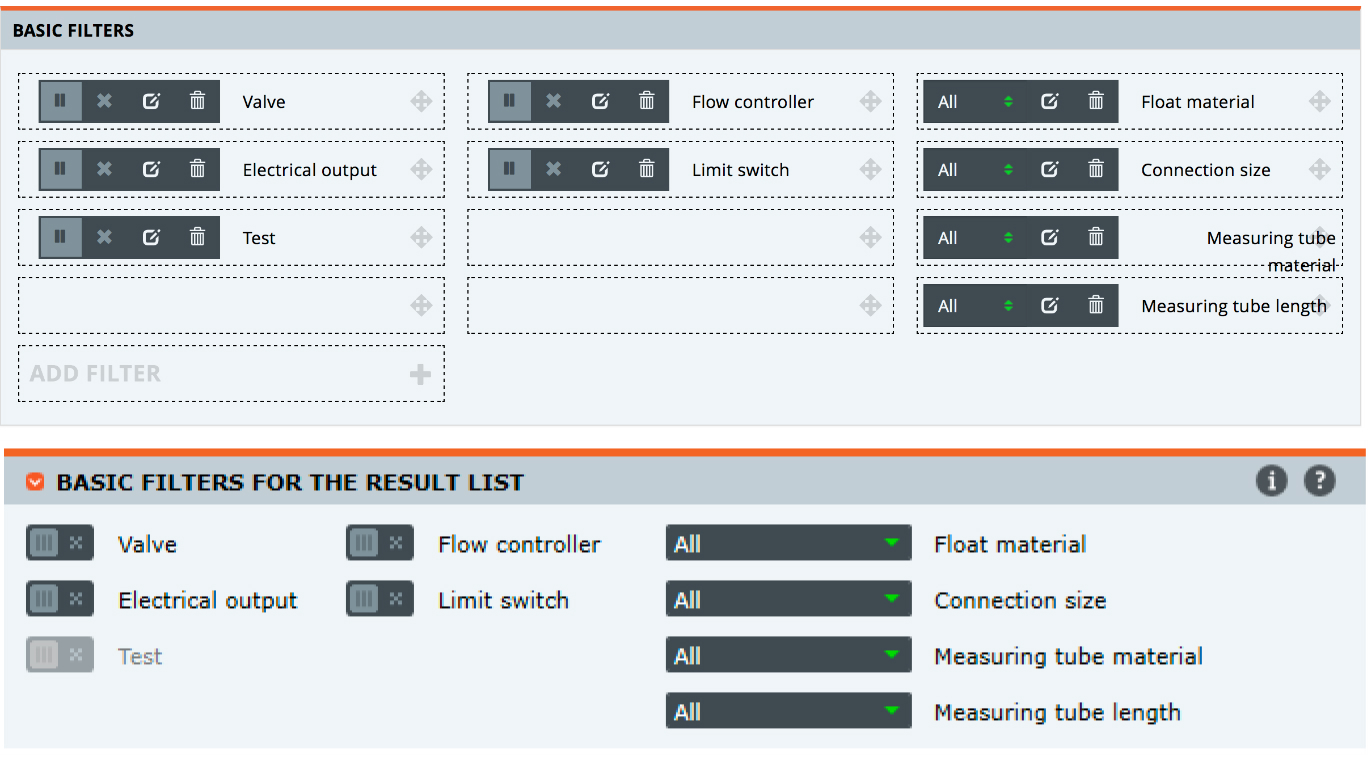
\includegraphics[width=1.0\textwidth]{testergebnis} %{CS0031}
\caption{Vergleich der Webanwendung und FlowConfigurator Software nach dem durchgeführten Integrationstest}
\label{fig:test}
\end{figure}

Auf dem Vergleichsbild lässt sich erkennen, dass der neu angelegte Testfilter, sowohl in der Webanwendung, als auch in der FlowConfigurator Software an der richtigen Stelle angezeigt wird. Auch wenn das entwickelte Testszenario formal alle aufgestellten funktionalen Anforderungen abdeckt und alle erwarteten Ergebnisse bestätigt werden konnten, kann das angewandte Testverfahren nur grob eine Aussage über die tatsächliche Funktionsfähigkeit der Webanwendung geben. Bei dem angewandten Testszenario handelt es sich zwar um die typische angedachte Benutzungsweise der Webanwendung, es wurden allerdings keine Randbedingungen untersucht. Abschließend lässt sich dennoch, auf Grundlage des durchgeführten Tests, die Behauptungen aufstellen, das mit dem entwickelten Prototypen, die am Anfang der Arbeit definierte Zielsetzung erreicht werden konnte.